\documentclass[presentation]{beamer}
\usepackage[utf8]{inputenc}
\usepackage[T1]{fontenc}
\usepackage{graphicx}
\usepackage{grffile}
\usepackage{longtable}
\usepackage{wrapfig}
\usepackage{rotating}
\usepackage[normalem]{ulem}
\usepackage{amsmath}
\usepackage{textcomp}
\usepackage{amssymb}
\usepackage{capt-of}
\usepackage{hyperref}
\newcommand{\inlinelatex}[1]{#1}
\usetheme[sectionpage=none, block=fill]{metropolis}
\title{Performance and Cost-Aware in HPC: A Network Interconnect Impact Assessment}
\author{
\large
\underline{Anderson Mattheus Maliszewski} \\
\small
Instituto de Informática\\
Universidade Federal do Rio Grande do Sul\\
}
\date{CMP223 Computer System Performance Analysis (2019/2) \\ December 9th, 2019}

\definecolor{Black}{RGB}{0,0,0}
\setbeamercolor{frametitle}{bg=Black}

\begin{document}

\maketitle

\begin{frame}{Introduction}
\vfill
Growing demand for computational power
\begin{itemize}
\item HPC
\item Clusters and "as a Service" cloud models
\end{itemize}
\pause \vfill
Communication characteristics vary
\begin{itemize}
\item Parallel programs have specific purposes
\item Bandwidth and latency sensitive
\end{itemize}
\pause \vfill
Network interconnection is one of the \alert{bottlenecks}
\begin{itemize}
\item High Performance interconnects - InfiniBand
\end{itemize}
\end{frame}

\begin{frame}{Motivation}
    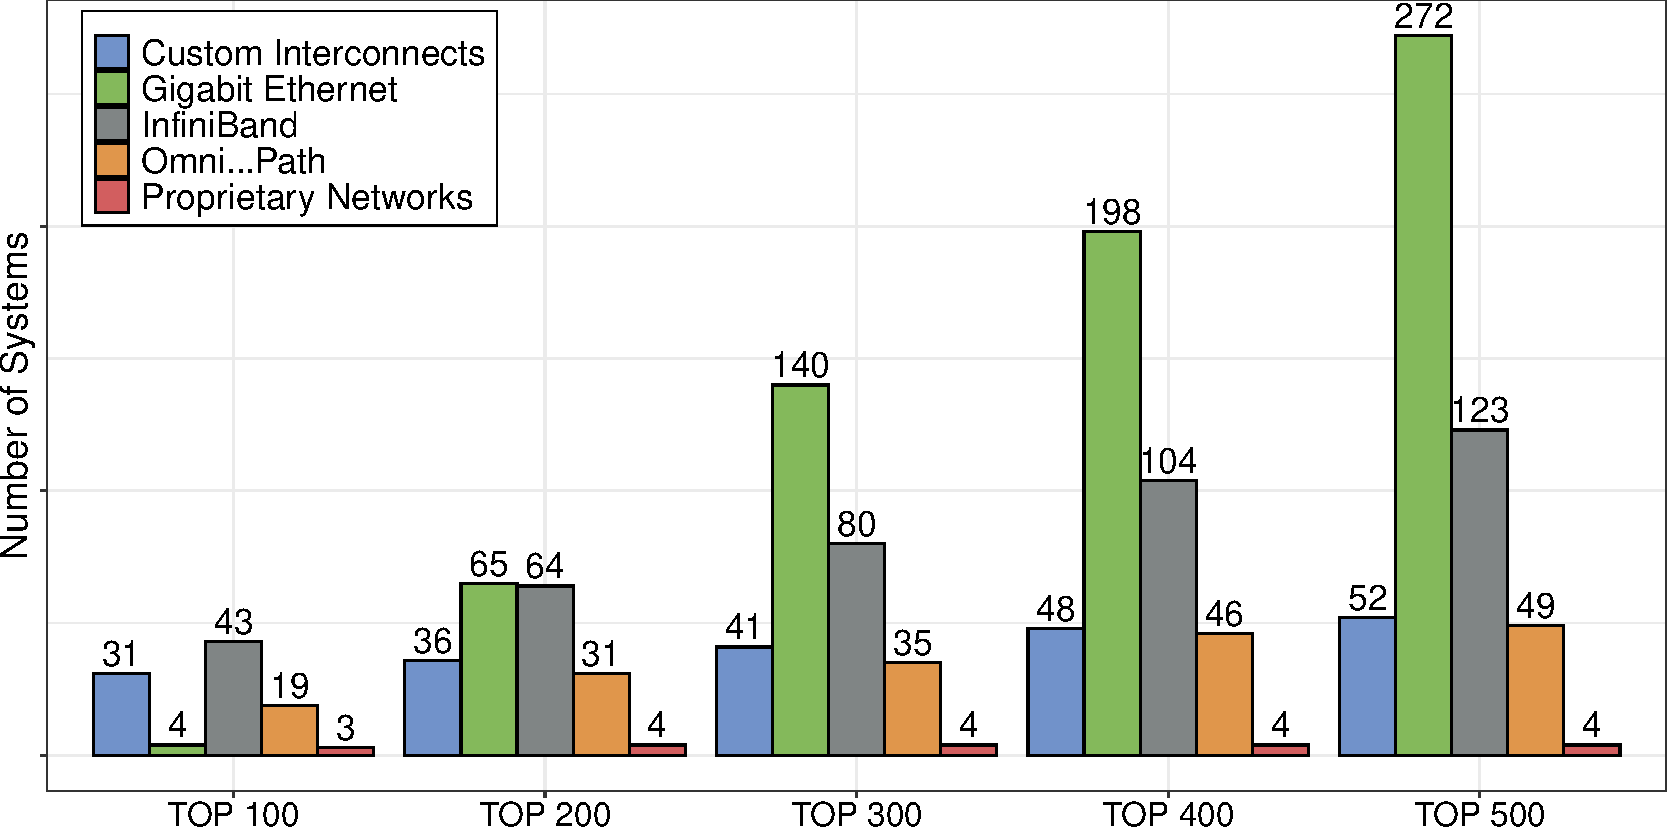
\includegraphics[width=\textwidth]{SLIDES/img/TOP500.pdf}
    %\includegraphics[width=.9\linewidth]{./img/reordering_example.png}
\end{frame}


\begin{frame}{Objective}
 \vfill
This work study the application \alert{\texttt{QR\_mumps}}, a parallel task-based
sparse QR factorization based on the \alert{multifrontal method}
\pause \vfill
We are interested in the performance analysis of the application
related to the \alert{ordering algorithms} and the \alert{elimination tree}
\pause \vfill
\begin{itemize}
\item Is an \alert{ordering} algorithm \alert{better than other}? 
\begin{itemize}
\item If so, why is it better?
\end{itemize}
\end{itemize}
\pause \vfill
\begin{itemize}
\item How the algorithm \alert{explores} the tree structure? 
\begin{itemize}
\item Does it impacts the performance?
\end{itemize}
\end{itemize}
\pause \vfill
\begin{itemize}
\item How \alert{memory constraints} impact performance?
\end{itemize}
\pause \vfill
To answer these questions, we will investigate and analyse the
application in different scenarios
\vfill
\end{frame}

\begin{frame}[fragile,label={sec:orge350978}]{Outline}
 \vfill
\Large
\begin{itemize}
\item Background
\begin{itemize}
\item Ordering and Fill-In
\item Elimination Tree
\item \texttt{QR\_mumps} and StarPU
\end{itemize}
\end{itemize}
\vfill
\begin{itemize}
\item Methodology
\begin{itemize}
\item Workload Characterization
\item Experimental Design
\end{itemize}
\end{itemize}
\vfill
\begin{itemize}
\item Results
\begin{itemize}
\item Ordering Impact
\item Interesting Cases Analysis
\end{itemize}
\end{itemize}
\vfill
\begin{itemize}
\item Conclusion
\end{itemize}
\begin{block}{}
\begin{center}
\Huge{Background}
\end{center}
\end{block}
\end{frame}
\begin{frame}[label={sec:org61a82f6}]{Ordering, Fill-In and Sparse Factorization}
\vfill
In the sparse factorization case, common dense factorization
strategies must be rethinked \footnote{[3] Van Loan C., Golub G. - Matrix Computations 4th Edition.} 
\vfill
\begin{itemize}
\item Sparse matrix \alert{data structure} for representation (COO, CSR)
\item \alert{Fill-in} reducing reordering
\end{itemize}
\vfill \pause
Operations may change the number of non-zeroes (NNZ), need to allocate
more space for these fill-ins
\vfill \pause
If we can \alert{predict} the positions that will be updated, we can add extra
space in the arrays for the representation of the matrix 
\end{frame}

\begin{frame}[label={sec:orgf91bff0}]{Ordering, Fill-In and Sparse Factorization}
\vfill
Commonly, the sparse factorization is preceeded by an \alert{analysis} step
\begin{itemize}
\item Permutate matrix rows and columns to reduce fill-in
\item Compute the matrix final structure (with fill-ins)
\end{itemize}
\vfill
Finding the \alert{optimal ordering} is a combinatorial problem
\vfill
Algorithms must use \alert{heuristics} to determine a good permutation of the
original matrix 
\vfill
\end{frame}

\begin{frame}[label={sec:orgbdefa6e}]{Ordering, Fill-In and Sparse Factorization}
In this case, the optimal ordering for the matrix allows to factorize
the matrix \alert{without introducing any fill-in}

%\begin{center}
%\includegraphics[width=.9\linewidth]{./img/reordering_example.png}
%\end{center}
\end{frame}

\begin{frame}[label={sec:orgcf1b76c}]{Elimination Tree}
\vfill
A good way to present sparse matrices is using graphs
\begin{itemize}
\item \alert{undirected} graphs are used to \alert{symmetric} matrices
\item \alert{directed} graphs for \alert{non-symmetric}
\end{itemize}
\vfill \pause
In the heart of the multifrontal method is the \alert{elimination tree}
\vfill
In its most common case, the tree has \alert{n} nodes, where n is the number
of columns of the input matrix problem
\vfill
Each node holds a denser submatrix called \alert{frontal matrix}
\vfill
Practical implementations group columns with similar structure into
\alert{supernodes} 
\vfill
\end{frame}
\begin{frame}[label={sec:orgf49f41b}]{Elimination Tree}
Example of a matrix and its elimination tree. The tree guides the
factorization 
\begin{columns}
\begin{column}{0.3\columnwidth}
\begin{center}
%\includegraphics[width=.9\linewidth]{./img/matrix_tree2.png}
\end{center}
\end{column}

\begin{column}{0.3\columnwidth}
\begin{center}
%\includegraphics[width=.9\linewidth]{./img/matrix_elimtree.png}
\end{center}
\end{column}
\end{columns}
\end{frame}
\begin{frame}[fragile,label={sec:orgb1800db}]{\texttt{QR\_mumps} and StarPU}
 \texttt{QR\_mumps} implements the multifrontal QR factorization
\begin{block}{}
\begin{center}
\Huge{Methodology}
\end{center}
\end{block}
\end{frame}
\begin{frame}[label={sec:org6435587}]{Workload Characterization}
\vfill
Before selecting our workloads, we listed some points that are
important to characterize our system workload: 
\begin{itemize}
\item Number of \alert{rows} and \alert{columns}
\item Non-zero Count (\alert{sparsity})
\item Shape of the matrix (tall, wide, square)
\end{itemize}
\vfill
We choose 10 matrices looking to explore different values
\vfill
They came from different problems: Linear Programming, Combinatorial
Problems, Economic Problems, Computational Simulation 
\vfill
\end{frame}
\begin{frame}[fragile,label={sec:orge4472a8}]{Workload Characterization}
 \newcommand{\ct}[1]{}
\setlength{\tabcolsep}{3pt}
\begin{table}[!h]
\caption{\label{tab:org3534e7a}
Workload matrices}
\centering
\begin{tabular}{lrrrll}
\hline
Name & Rows & Columns & NNZ & Sparsity & Problem\\
\hline
\texttt{karted} & 46.502 & 133.115 & 1.770.349 & 0,0285\% & L.P.\\
\texttt{TF18} & 95.368 & 123.867 & 1.597.545 & 0,0135\% & Comb.\\
\texttt{EternityII\_E} & 11.077 & 262.144 & 1.503.732 & 0,0517\% & Opt.\\
\hline
\texttt{g7jac200} & 59.310 & 59.310 & 837.936 & 0,0238\% & Ec.\\
\texttt{mk13-b5} & 135.135 & 270.270 & 810.810 & 0,0022\% & Comb.\\
\texttt{n4c6-b6} & 104.115 & 51.813 & 728.805 & 0,0135\% & Comb.\\
\hline
\texttt{ch8-8-b3} & 117.600 & 18.816 & 470.400 & 0,0212\% & Comb.\\
\texttt{flower\_8\_4} & 55.081 & 125.361 & 375.266 & 0,0054\% & Comb.\\
\texttt{fxm3\_16} & 41.340 & 85.575 & 392.252 & 0,0110\% & L.P.\\
\texttt{RAFEM\_16} & 16.729 & 16.729 & 450.450 & 0,0016\% & Sim.\\
\hline
\end{tabular}
\end{table}
\end{frame}

\begin{frame}[label={sec:orgee2da1f}]{Experimental Design}
\vfill
The experimental design follows a \alert{2\(^{\text{k}}\)} factorial design, \alert{k factors}
varying at \alert{two levels} for each matrix  
\begin{itemize}
\item Ordering algorithm: \alert{Metis} and \alert{Scotch}
\item Memory factor: \alert{Unlimited} and \alert{Sequential Peak}
\end{itemize}
\vfill
Workload selection:
\begin{itemize}
\item all 10 matrices
\end{itemize}
\vfill
Computational Environment
\begin{itemize}
\item 2 \texttimes{} Intel Xeon E5-2650 v3 (Q3'14) Haswell, 2.3 GHz
\item 20 núcleos (10 por CPU)
\item 128 GB DDR4 RAM
\end{itemize}
\vfill
\end{frame}

\begin{frame}[label={sec:org1898a0c}]{Experimental Design}
\vfill
The experimental design follows a \alert{2\(^{\text{kr}}\)} factorial design, \alert{k factors}
varying at \alert{two levels} for each matrix with \alert{30 or 10 repetitions}
\begin{itemize}
\item 30 repetitions for fast matrices and 10 for slower ones
\end{itemize}
\vfill
The objective of this experiment was to find \alert{interesting cases}
\begin{enumerate}
\item There are cases where the ordering changes the performance?
\begin{itemize}
\item Factorization time
\item Estimated total floating point operations
\item Memory peak consumption
\end{itemize}
\item There are cases where memory factor changes the performance?
\begin{itemize}
\item Memory peak
\item Ready and Submitted tasks
\item Active nodes
\end{itemize}
\item The ordering does not change performance at all
\end{enumerate}


\vfill
\end{frame}
\begin{frame}[label={sec:org7b38ff4}]{}
\begin{center}
\Huge{Results}
\end{center}
\end{frame}
\begin{frame}[label={sec:orga503c53}]{Evaluating The Ordering Impact on Performance}
\end{frame}
\begin{frame}[label={sec:orge83a529}]{Analysis Of Interesting Cases}
\end{frame}
\begin{frame}[label={sec:org4d8e86e}]{Ordering Impact}
\end{frame}
\begin{frame}[label={sec:org003c168}]{Interesting Case Analysis}
\end{frame}
\begin{frame}[label={sec:org09ae9aa}]{Conclusion}
\end{frame}
\begin{frame}[label={sec:orgcc17679}]{References}
\footnotesize{[1] P. R. Amestoy, I. S. Duff, and J.-Y. L’excellent, “Multifrontal parallel
distributed symmetric and unsymmetric solvers,” Computer methods in applied mechanics and
engineering, vol. 184, no. 2-4, pp. 501–520, 2000.}

\footnotesize{[2] J. W. Liu, “The role of elimination trees in sparse factorization,”
SIAM journal on matrix analysis and applications, vol. 11, no. 1, pp. 134–172, 1990.}

\footnotesize{[3] Van Loan, Charles F.; Golub, Gene H. Matrix computations. Johns Hopkins
University Press, 1983.}
\end{frame}
\begin{frame}[label={sec:orgd50d830}]{}
\begin{center}
\Huge{Thank You!}

\newline

\Large{marcelo.miletto@inf.ufrgs.br}
\end{center}
\end{frame}
\end{document}